\documentclass[twoside]{book}

% Packages required by doxygen
\usepackage{fixltx2e}
\usepackage{calc}
\usepackage{doxygen}
\usepackage[export]{adjustbox} % also loads graphicx
\usepackage{graphicx}
\usepackage[utf8]{inputenc}
\usepackage{makeidx}
\usepackage{multicol}
\usepackage{multirow}
\PassOptionsToPackage{warn}{textcomp}
\usepackage{textcomp}
\usepackage[nointegrals]{wasysym}
\usepackage[table]{xcolor}

% Font selection
\usepackage[T1]{fontenc}
\usepackage[scaled=.90]{helvet}
\usepackage{courier}
\usepackage{amssymb}
\usepackage{sectsty}
\renewcommand{\familydefault}{\sfdefault}
\allsectionsfont{%
  \fontseries{bc}\selectfont%
  \color{darkgray}%
}
\renewcommand{\DoxyLabelFont}{%
  \fontseries{bc}\selectfont%
  \color{darkgray}%
}
\newcommand{\+}{\discretionary{\mbox{\scriptsize$\hookleftarrow$}}{}{}}

% Page & text layout
\usepackage{geometry}
\geometry{%
  a4paper,%
  top=2.5cm,%
  bottom=2.5cm,%
  left=2.5cm,%
  right=2.5cm%
}
\tolerance=750
\hfuzz=15pt
\hbadness=750
\setlength{\emergencystretch}{15pt}
\setlength{\parindent}{0cm}
\setlength{\parskip}{0.2cm}
\makeatletter
\renewcommand{\paragraph}{%
  \@startsection{paragraph}{4}{0ex}{-1.0ex}{1.0ex}{%
    \normalfont\normalsize\bfseries\SS@parafont%
  }%
}
\renewcommand{\subparagraph}{%
  \@startsection{subparagraph}{5}{0ex}{-1.0ex}{1.0ex}{%
    \normalfont\normalsize\bfseries\SS@subparafont%
  }%
}
\makeatother

% Headers & footers
\usepackage{fancyhdr}
\pagestyle{fancyplain}
\fancyhead[LE]{\fancyplain{}{\bfseries\thepage}}
\fancyhead[CE]{\fancyplain{}{}}
\fancyhead[RE]{\fancyplain{}{\bfseries\leftmark}}
\fancyhead[LO]{\fancyplain{}{\bfseries\rightmark}}
\fancyhead[CO]{\fancyplain{}{}}
\fancyhead[RO]{\fancyplain{}{\bfseries\thepage}}
\fancyfoot[LE]{\fancyplain{}{}}
\fancyfoot[CE]{\fancyplain{}{}}
\fancyfoot[RE]{\fancyplain{}{\bfseries\scriptsize Generated on Thu Aug 4 2016 14\+:07\+:52 for func\+\_\+test by Doxygen }}
\fancyfoot[LO]{\fancyplain{}{\bfseries\scriptsize Generated on Thu Aug 4 2016 14\+:07\+:52 for func\+\_\+test by Doxygen }}
\fancyfoot[CO]{\fancyplain{}{}}
\fancyfoot[RO]{\fancyplain{}{}}
\renewcommand{\footrulewidth}{0.4pt}
\renewcommand{\chaptermark}[1]{%
  \markboth{#1}{}%
}
\renewcommand{\sectionmark}[1]{%
  \markright{\thesection\ #1}%
}

% Indices & bibliography
\usepackage{natbib}
\usepackage[titles]{tocloft}
\setcounter{tocdepth}{3}
\setcounter{secnumdepth}{5}
\makeindex

% Hyperlinks (required, but should be loaded last)
\usepackage{ifpdf}
\ifpdf
  \usepackage[pdftex,pagebackref=true]{hyperref}
\else
  \usepackage[ps2pdf,pagebackref=true]{hyperref}
\fi
\hypersetup{%
  colorlinks=true,%
  linkcolor=blue,%
  citecolor=blue,%
  unicode%
}

% Custom commands
\newcommand{\clearemptydoublepage}{%
  \newpage{\pagestyle{empty}\cleardoublepage}%
}


%===== C O N T E N T S =====

\begin{document}

% Titlepage & ToC
\hypersetup{pageanchor=false,
             bookmarks=true,
             bookmarksnumbered=true,
             pdfencoding=unicode
            }
\pagenumbering{roman}
\begin{titlepage}
\vspace*{7cm}
\begin{center}%
{\Large func\+\_\+test \\[1ex]\large master }\\
\vspace*{1cm}
{\large Generated by Doxygen 1.8.10}\\
\vspace*{0.5cm}
{\small Thu Aug 4 2016 14:07:52}\\
\end{center}
\end{titlepage}
\clearemptydoublepage
\tableofcontents
\clearemptydoublepage
\pagenumbering{arabic}
\hypersetup{pageanchor=true}

%--- Begin generated contents ---
\chapter{Deprecated List}
\label{deprecated}
\hypertarget{deprecated}{}

\begin{DoxyRefList}
\item[\label{deprecated__deprecated000001}%
\hypertarget{deprecated__deprecated000001}{}%
global\+Scope$>$ Global \hyperlink{group___function_ga59ab1d2d44475cf677d4025aedfc22ea}{function} (void)]
\item[\label{deprecated__deprecated000002}%
\hypertarget{deprecated__deprecated000002}{}%
global\+Scope$>$ Global \hyperlink{group___function_ga05848de25ac2dbec233935058a1d24b4}{init} ()]
\end{DoxyRefList}
\chapter{Module Index}
\section{Modules}
Here is a list of all modules\+:\begin{DoxyCompactList}
\item \contentsline{section}{Function}{\pageref{group___function}}{}
\item \contentsline{section}{M\+O\+D\+U\+L\+E\+S\+\_\+\+Exported\+\_\+\+Types}{\pageref{group___m_o_d_u_l_e_s___exported___types}}{}
\end{DoxyCompactList}

\chapter{Data Structure Index}
\section{Data Structures}
Here are the data structures with brief descriptions\+:\begin{DoxyCompactList}
\item\contentsline{section}{\hyperlink{struct_f_u_n_c___expo_type_def}{F\+U\+N\+C\+\_\+\+Expo\+Type\+Def} \\*\hyperlink{struct_f_u_n_c___expo_type_def}{F\+U\+N\+C\+\_\+\+Expo\+Type\+Def} structure definition }{\pageref{struct_f_u_n_c___expo_type_def}}{}
\end{DoxyCompactList}

\chapter{File Index}
\section{File List}
Here is a list of all documented files with brief descriptions\+:\begin{DoxyCompactList}
\item\contentsline{section}{D\+:/workspace/doxygen/function/src/\hyperlink{function_8c}{function.\+c} \\*Main function-\/config-\/init-\/loop schedule }{\pageref{function_8c}}{}
\item\contentsline{section}{D\+:/workspace/doxygen/function/src/\hyperlink{function_8h}{function.\+h} \\*This file contains all the functions prototypes for the funtion.\+c }{\pageref{function_8h}}{}
\end{DoxyCompactList}

\chapter{Module Documentation}
\hypertarget{group___function}{}\section{Function}
\label{group___function}\index{Function@{Function}}
\subsection*{Functions}
\begin{DoxyCompactItemize}
\item 
int \hyperlink{group___function_ga05848de25ac2dbec233935058a1d24b4}{init} ()
\begin{DoxyCompactList}\small\item\em Function descreption. \end{DoxyCompactList}\item 
int \hyperlink{group___function_ga59ab1d2d44475cf677d4025aedfc22ea}{function} (void)
\begin{DoxyCompactList}\small\item\em This function exception. \end{DoxyCompactList}\end{DoxyCompactItemize}


\subsection{Detailed Description}


\subsection{Function Documentation}
\hypertarget{group___function_ga59ab1d2d44475cf677d4025aedfc22ea}{}\index{Function@{Function}!function@{function}}
\index{function@{function}!Function@{Function}}
\subsubsection[{function(void)}]{\setlength{\rightskip}{0pt plus 5cm}int function (
\begin{DoxyParamCaption}
\item[{void}]{}
\end{DoxyParamCaption}
)}\label{group___function_ga59ab1d2d44475cf677d4025aedfc22ea}


This function exception. 


\begin{DoxyParams}[1]{Parameters}
\mbox{\tt in}  & {\em None} & \\
\hline
\mbox{\tt out}  & {\em None} & \\
\hline
\end{DoxyParams}
\begin{DoxyReturn}{Returns}
int 
\end{DoxyReturn}
\begin{DoxyNote}{Note}

\end{DoxyNote}
\begin{DoxyParagraph}{}

\begin{DoxyCode}
1 int ret = init();
\end{DoxyCode}
 
\end{DoxyParagraph}
\begin{DoxySeeAlso}{See also}

\end{DoxySeeAlso}
\begin{DoxyRefDesc}{Deprecated}
\item[\hyperlink{deprecated__deprecated000001}{Deprecated}]\end{DoxyRefDesc}


Here is the call graph for this function\+:\nopagebreak
\begin{figure}[H]
\begin{center}
\leavevmode
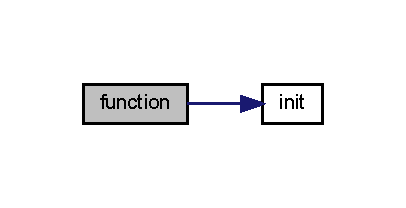
\includegraphics[width=195pt]{group___function_ga59ab1d2d44475cf677d4025aedfc22ea_cgraph}
\end{center}
\end{figure}


\hypertarget{group___function_ga05848de25ac2dbec233935058a1d24b4}{}\index{Function@{Function}!init@{init}}
\index{init@{init}!Function@{Function}}
\subsubsection[{init()}]{\setlength{\rightskip}{0pt plus 5cm}int init (
\begin{DoxyParamCaption}
\item[{void}]{}
\end{DoxyParamCaption}
)}\label{group___function_ga05848de25ac2dbec233935058a1d24b4}


Function descreption. 

This function exception.


\begin{DoxyParams}[1]{Parameters}
\mbox{\tt in}  & {\em None} & \\
\hline
\mbox{\tt out}  & {\em None} & \\
\hline
\end{DoxyParams}
\begin{DoxyReturn}{Returns}
int 
\end{DoxyReturn}
\begin{DoxyNote}{Note}

\end{DoxyNote}
\begin{DoxyParagraph}{}

\begin{DoxyCode}
1 int ret = init();
\end{DoxyCode}
 
\end{DoxyParagraph}
\begin{DoxySeeAlso}{See also}

\end{DoxySeeAlso}
\begin{DoxyRefDesc}{Deprecated}
\item[\hyperlink{deprecated__deprecated000002}{Deprecated}]\end{DoxyRefDesc}


Here is the caller graph for this function\+:\nopagebreak
\begin{figure}[H]
\begin{center}
\leavevmode
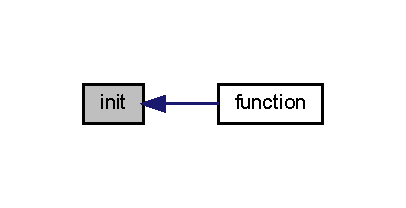
\includegraphics[width=195pt]{group___function_ga05848de25ac2dbec233935058a1d24b4_icgraph}
\end{center}
\end{figure}



\hypertarget{group___m_o_d_u_l_e_s___exported___types}{}\section{M\+O\+D\+U\+L\+E\+S\+\_\+\+Exported\+\_\+\+Types}
\label{group___m_o_d_u_l_e_s___exported___types}\index{M\+O\+D\+U\+L\+E\+S\+\_\+\+Exported\+\_\+\+Types@{M\+O\+D\+U\+L\+E\+S\+\_\+\+Exported\+\_\+\+Types}}
\subsection*{Data Structures}
\begin{DoxyCompactItemize}
\item 
struct \hyperlink{struct_f_u_n_c___expo_type_def}{F\+U\+N\+C\+\_\+\+Expo\+Type\+Def}
\begin{DoxyCompactList}\small\item\em \hyperlink{struct_f_u_n_c___expo_type_def}{F\+U\+N\+C\+\_\+\+Expo\+Type\+Def} structure definition. \end{DoxyCompactList}\end{DoxyCompactItemize}


\subsection{Detailed Description}

\chapter{Data Structure Documentation}
\hypertarget{struct_f_u_n_c___expo_type_def}{}\section{F\+U\+N\+C\+\_\+\+Expo\+Type\+Def Struct Reference}
\label{struct_f_u_n_c___expo_type_def}\index{F\+U\+N\+C\+\_\+\+Expo\+Type\+Def@{F\+U\+N\+C\+\_\+\+Expo\+Type\+Def}}


\hyperlink{struct_f_u_n_c___expo_type_def}{F\+U\+N\+C\+\_\+\+Expo\+Type\+Def} structure definition.  




{\ttfamily \#include $<$function.\+h$>$}

\subsection*{Data Fields}
\begin{DoxyCompactItemize}
\item 
uint32\+\_\+t \hyperlink{struct_f_u_n_c___expo_type_def_a814e9c0a2e62eaea6c35bc6d701232d2}{F\+U\+N\+C\+\_\+\+Mode}
\item 
Functional\+State \hyperlink{struct_f_u_n_c___expo_type_def_a107ceb2119e7b259a591eef448594980}{F\+U\+N\+C\+\_\+\+Scan\+Conv\+Mode}
\end{DoxyCompactItemize}


\subsection{Detailed Description}
\hyperlink{struct_f_u_n_c___expo_type_def}{F\+U\+N\+C\+\_\+\+Expo\+Type\+Def} structure definition. 

\subsection{Field Documentation}
\hypertarget{struct_f_u_n_c___expo_type_def_a814e9c0a2e62eaea6c35bc6d701232d2}{}\index{F\+U\+N\+C\+\_\+\+Expo\+Type\+Def@{F\+U\+N\+C\+\_\+\+Expo\+Type\+Def}!F\+U\+N\+C\+\_\+\+Mode@{F\+U\+N\+C\+\_\+\+Mode}}
\index{F\+U\+N\+C\+\_\+\+Mode@{F\+U\+N\+C\+\_\+\+Mode}!F\+U\+N\+C\+\_\+\+Expo\+Type\+Def@{F\+U\+N\+C\+\_\+\+Expo\+Type\+Def}}
\subsubsection[{F\+U\+N\+C\+\_\+\+Mode}]{\setlength{\rightskip}{0pt plus 5cm}uint32\+\_\+t F\+U\+N\+C\+\_\+\+Mode}\label{struct_f_u_n_c___expo_type_def_a814e9c0a2e62eaea6c35bc6d701232d2}
Configures the A\+D\+C to operate in independent or dual mode. This parameter can be a value of A\+D\+C\+\_\+mode \hypertarget{struct_f_u_n_c___expo_type_def_a107ceb2119e7b259a591eef448594980}{}\index{F\+U\+N\+C\+\_\+\+Expo\+Type\+Def@{F\+U\+N\+C\+\_\+\+Expo\+Type\+Def}!F\+U\+N\+C\+\_\+\+Scan\+Conv\+Mode@{F\+U\+N\+C\+\_\+\+Scan\+Conv\+Mode}}
\index{F\+U\+N\+C\+\_\+\+Scan\+Conv\+Mode@{F\+U\+N\+C\+\_\+\+Scan\+Conv\+Mode}!F\+U\+N\+C\+\_\+\+Expo\+Type\+Def@{F\+U\+N\+C\+\_\+\+Expo\+Type\+Def}}
\subsubsection[{F\+U\+N\+C\+\_\+\+Scan\+Conv\+Mode}]{\setlength{\rightskip}{0pt plus 5cm}Functional\+State F\+U\+N\+C\+\_\+\+Scan\+Conv\+Mode}\label{struct_f_u_n_c___expo_type_def_a107ceb2119e7b259a591eef448594980}
Specifies whether the conversion is performed in Scan (multichannels) or Single (one channel) mode. This parameter can be set to E\+N\+A\+B\+L\+E or D\+I\+S\+A\+B\+L\+E 

The documentation for this struct was generated from the following file\+:\begin{DoxyCompactItemize}
\item 
D\+:/workspace/doxygen/function/src/\hyperlink{function_8h}{function.\+h}\end{DoxyCompactItemize}

\chapter{File Documentation}
\hypertarget{function_8c}{}\section{D\+:/workspace/doxygen/function/src/function.c File Reference}
\label{function_8c}\index{D\+:/workspace/doxygen/function/src/function.\+c@{D\+:/workspace/doxygen/function/src/function.\+c}}


main function-\/config-\/init-\/loop schedule  


{\ttfamily \#include \char`\"{}function.\+h\char`\"{}}\\*
Include dependency graph for function.\+c\+:
\nopagebreak
\begin{figure}[H]
\begin{center}
\leavevmode
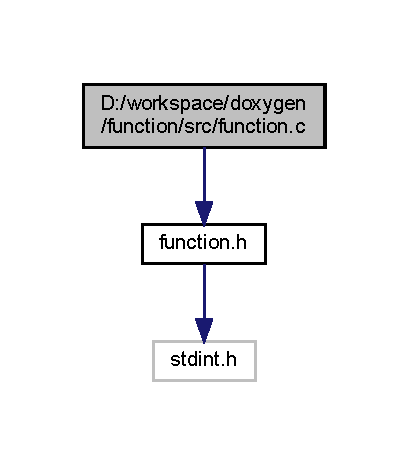
\includegraphics[width=196pt]{function_8c__incl}
\end{center}
\end{figure}
\subsection*{Functions}
\begin{DoxyCompactItemize}
\item 
int \hyperlink{group___function_ga05848de25ac2dbec233935058a1d24b4}{init} ()
\begin{DoxyCompactList}\small\item\em Function descreption. \end{DoxyCompactList}\item 
int \hyperlink{group___function_ga59ab1d2d44475cf677d4025aedfc22ea}{function} (void)
\begin{DoxyCompactList}\small\item\em This function exception. \end{DoxyCompactList}\end{DoxyCompactItemize}


\subsection{Detailed Description}
main function-\/config-\/init-\/loop schedule 

\begin{DoxyAuthor}{Author}
I\+W\+O\+S2610 
\end{DoxyAuthor}
\begin{DoxyVersion}{Version}
V1.\+0.\+0 
\end{DoxyVersion}
\begin{DoxyDate}{Date}
2016-\/08-\/03 
\end{DoxyDate}
\begin{DoxyAttention}{Attention}

\end{DoxyAttention}
N\+O

\subsubsection*{\begin{center}\copyright{} C\+O\+P\+Y\+R\+I\+G\+H\+T 2016 I\+W\+O\+S2610 \end{center} }
\hypertarget{function_8h}{}\section{D\+:/workspace/doxygen/function/src/function.h File Reference}
\label{function_8h}\index{D\+:/workspace/doxygen/function/src/function.\+h@{D\+:/workspace/doxygen/function/src/function.\+h}}


This file contains all the functions prototypes for the funtion.\+c.  


{\ttfamily \#include \char`\"{}stdint.\+h\char`\"{}}\\*
Include dependency graph for function.\+h\+:
\nopagebreak
\begin{figure}[H]
\begin{center}
\leavevmode
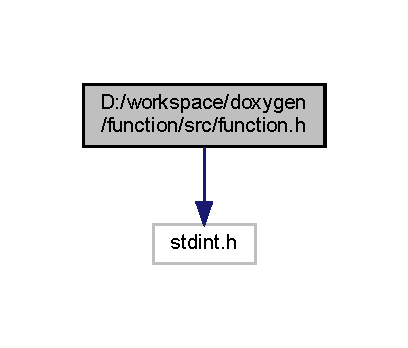
\includegraphics[width=196pt]{function_8h__incl}
\end{center}
\end{figure}
This graph shows which files directly or indirectly include this file\+:
\nopagebreak
\begin{figure}[H]
\begin{center}
\leavevmode
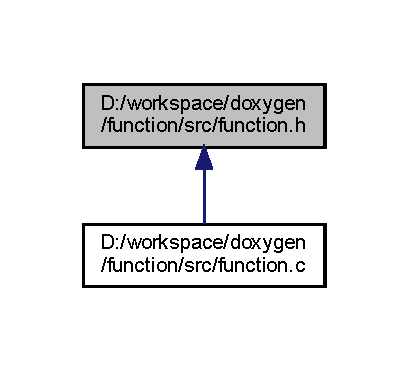
\includegraphics[width=196pt]{function_8h__dep__incl}
\end{center}
\end{figure}
\subsection*{Data Structures}
\begin{DoxyCompactItemize}
\item 
struct \hyperlink{struct_f_u_n_c___expo_type_def}{F\+U\+N\+C\+\_\+\+Expo\+Type\+Def}
\begin{DoxyCompactList}\small\item\em \hyperlink{struct_f_u_n_c___expo_type_def}{F\+U\+N\+C\+\_\+\+Expo\+Type\+Def} structure definition. \end{DoxyCompactList}\end{DoxyCompactItemize}
\subsection*{Macros}
{\bf }\par
\begin{DoxyCompactItemize}
\item 
\#define \hyperlink{function_8h_a0a4f7bda268774b0e59df907ea41223e}{I\+W\+O\+S2610}~(0x2610)
\end{DoxyCompactItemize}

\subsection*{Functions}
\begin{DoxyCompactItemize}
\item 
int \hyperlink{group___function_ga59ab1d2d44475cf677d4025aedfc22ea}{function} (void)
\begin{DoxyCompactList}\small\item\em This function exception. \end{DoxyCompactList}\end{DoxyCompactItemize}


\subsection{Detailed Description}
This file contains all the functions prototypes for the funtion.\+c. 

\begin{DoxyAuthor}{Author}
I\+W\+O\+S2610 
\end{DoxyAuthor}
\begin{DoxyVersion}{Version}
V1.\+0.\+0 
\end{DoxyVersion}
\begin{DoxyDate}{Date}
2016-\/08-\/03 
\end{DoxyDate}
\begin{DoxyAttention}{Attention}

\end{DoxyAttention}
N\+O

\subsubsection*{\begin{center}\copyright{} C\+O\+P\+Y\+R\+I\+G\+H\+T 2016 I\+W\+O\+S2610 \end{center} }

\subsection{Macro Definition Documentation}
\hypertarget{function_8h_a0a4f7bda268774b0e59df907ea41223e}{}\index{function.\+h@{function.\+h}!I\+W\+O\+S2610@{I\+W\+O\+S2610}}
\index{I\+W\+O\+S2610@{I\+W\+O\+S2610}!function.\+h@{function.\+h}}
\subsubsection[{I\+W\+O\+S2610}]{\setlength{\rightskip}{0pt plus 5cm}\#define I\+W\+O\+S2610~(0x2610)}\label{function_8h_a0a4f7bda268774b0e59df907ea41223e}
to group Function 
%--- End generated contents ---

% Index
\backmatter
\newpage
\phantomsection
\clearemptydoublepage
\addcontentsline{toc}{chapter}{Index}
\printindex

\end{document}
